
\begin{table}[H]
\begin{flushleft}\emph{\textbf{Use Case}}\end{flushleft}
\footnotesize
\centering
\settowidth\tymin{\textbf{Entry conditions}}
\setlength\extrarowheight{2pt}
\begin{tabulary}{\textwidth}{|J|J|}
\hline
Name  & View Safety \\
\hline
Actor & Registered User \\
\hline
Entry conditions & The user wants to check the safety of a certain area that he is interested in \\
\hline
Events flow & 
\begin{minipage}[t]{0.7\textwidth}
\begin{enumerate} 
\item In the homepage the user opens the view safety section of the app
\item The user specifies details of the area he is interested in
\item The user submits search criteria and chooses area from a list of matches
\item The user is represented with a geographical representation of the area’s safety based on number of violations and accidents occurring in the area
\end{enumerate}
\end{minipage}\\
\hline
Exit conditions  & The user is represented with area safety\\
\hline
Exceptions       & 
\begin{minipage}[t]{0.8\textwidth}
\begin{itemize} 
\item The specified area does not yield any search results: A message stating there are no results matching entered data is shown
\end{itemize}
\end{minipage}\\
\hline
\end{tabulary}
\caption{\label{tab:Usecase-View-Safety}Usecase for View Safety}
\end{table}

The following figure describes the view safety process. In which, the user is able to see a representation of the safety of various areas based on their search. The user enters the area details and if there are any reports in that area a geographical representation of the area is shown.

\begin{figure}[H]
\begin{flushleft}\emph{\textbf{Sequence Diagram}}\end{flushleft}
\caption{Sequence Diagram for View Safety}
\label{fig:SD-View-Safety}
\centering
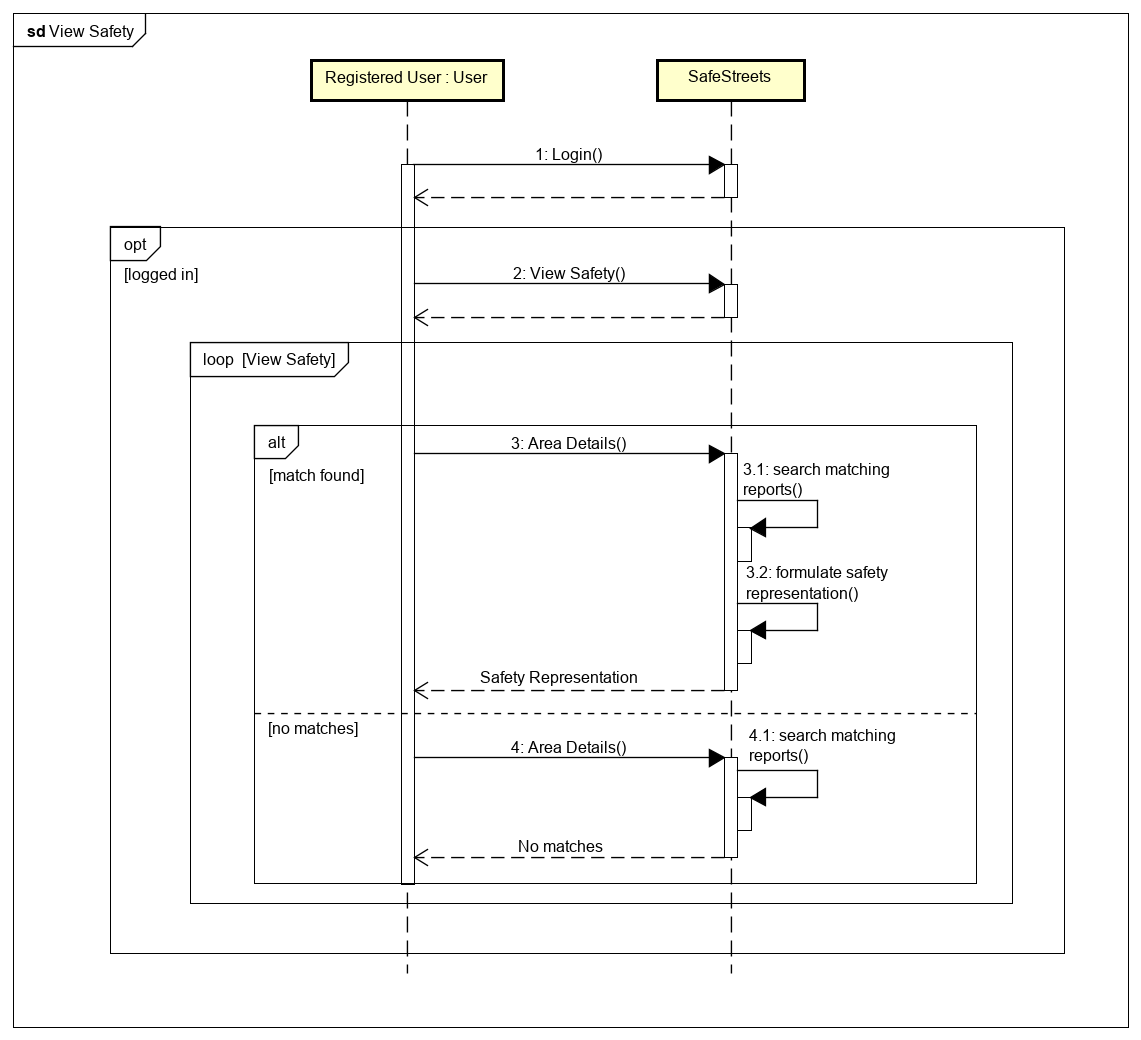
\includegraphics[width=\textwidth, height=0.90\textheight]{view-safety-SD.png}
\end{figure}


%***place holder for report-violation-sd***
